\documentclass[aspectratio=169, table, 12pt]{beamer}

\usepackage{colortbl}
\usepackage{xcolor}
\usepackage{listings}
\usepackage{tabularx}
\usepackage{tikz}
\usetikzlibrary{arrows.meta, positioning, calc, fit, shapes.geometric}

\makeatletter
\def\input@path{{../theme/}}
\makeatother
\graphicspath{{../theme/}{../../figures/}}
\usetheme{Pradita}

\definecolor{praditagreen}{RGB}{37, 113, 71}

% Tema membuat garis tabel berwarna putih. Dikembalikan agar tabel terbaca.
\arrayrulecolor{black}
\setlength{\arrayrulewidth}{0.5pt}

\lstdefinestyle{PythonStyle}{
  language=Python,
  basicstyle=\ttfamily\scriptsize,
  keywordstyle=\color{blue}\bfseries,
  commentstyle=\color{gray}\itshape,
  stringstyle=\color{red},
  breaklines=true,
  frame=lines,
  backgroundcolor=\color{lightgray!10},
  tabsize=2,
  showstringspaces=false
}

\lstdefinelanguage{bash}{
  keywords={},
  basicstyle=\ttfamily\scriptsize,
  ndkeywords={cd, python},
  ndkeywordstyle=\color{purple}\bfseries,
  sensitive=true,
  commentstyle=\color{gray},
  breaklines=true,
  frame=lines,
  backgroundcolor=\color{lightgray!10},
  tabsize=2,
  comment=[l]{\#},
  showstringspaces=false
}

\title{\LARGE{Pertemuan 04:}\\ \Huge{Ports and Adapters}}
\subtitle{IF231303 Arsitektur Perangkat Lunak}
\author{Alfa Yohannis}

\begin{document}

\frame{\titlepage}

\begin{frame}{{\Large Tujuan Pembelajaran}}
  \vspace{10pt}
  \begin{enumerate}
    \item Menjelaskan peran port dan adapter serta arah ketergantungan yang
          membuat logika inti bebas dari teknologi penyimpanan.
    \item Membedakan port masukan dari port keluaran.
    \item Mengukur kemandirian logika inti, biaya penggantian adapter, dan
          cakupan pengujian tanpa infrastruktur.
  \end{enumerate}
\end{frame}

\begin{frame}{{\Large Masalah yang Tersisa dari Bab 2}}
  \vspace{10pt}
  \begin{itemize}
    \item Layered menjaga arah panggilan tetap ke bawah.
    \item Aturan itu menahan perubahan di satu lapisan.
    \item Namun lapisan bisnis tetap memanggil lapisan persistensi.
    \item Artinya logika inti tetap mengenal keberadaan penyimpanan.
  \end{itemize}

  \vspace{10pt}
  {\small Ports and adapters menyelesaikannya dengan membalik arah
  ketergantungan.}
\end{frame}

\begin{frame}{{\Large Seluruh Panah Menunjuk ke Dalam}}
  \vspace{5pt}
  \centering
  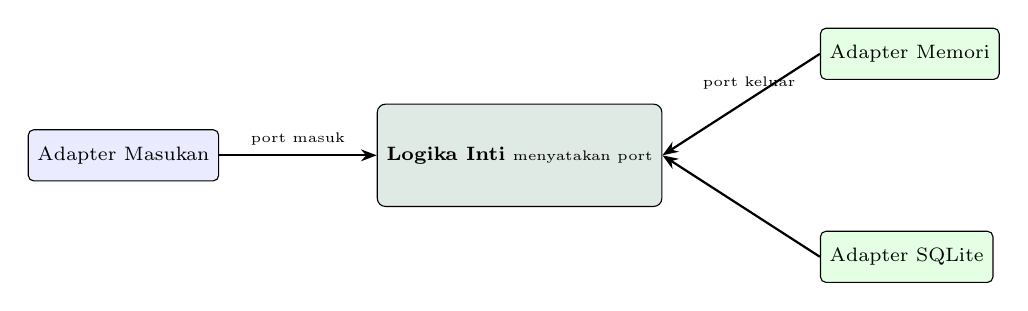
\begin{tikzpicture}[
    kotak/.style={draw, rounded corners=2pt, minimum width=2.0cm,
      minimum height=0.65cm, align=center, font=\scriptsize},
    inti/.style={draw, rounded corners=3pt, minimum width=3.0cm,
      minimum height=1.3cm, align=center, font=\scriptsize, fill=praditagreen!15},
    panah/.style={-{Stealth[length=2mm]}, thick}
  ]
    \node[inti] (inti) {\textbf{Logika Inti}
      {\tiny\mdseries menyatakan port}};
    \node[kotak, fill=blue!8, left=2.0cm of inti] (masuk) {Adapter Masukan};
    \node[kotak, fill=green!10, above right=0.3cm and 2.0cm of inti] (memori) {Adapter Memori};
    \node[kotak, fill=green!10, below right=0.3cm and 2.0cm of inti] (sqlite) {Adapter SQLite};
    \draw[panah] (masuk) -- node[above, font=\tiny] {port masuk} (inti);
    \draw[panah] (memori.west) -- node[above, font=\tiny, pos=0.45] {port keluar} (inti.east);
    \draw[panah] (sqlite.west) -- (inti.east);
  \end{tikzpicture}

  \vspace{8pt}
  {\small Satu port dapat diisi banyak adapter sekaligus.}
\end{frame}

\begin{frame}[fragile]{{\Large Port Ditulis oleh Logika Inti}}
  \vspace{5pt}
\begin{lstlisting}[style=PythonStyle]
class SumberKurs(Protocol):
  # Port keluaran yang dibutuhkan logika inti. Siapa pun yang menyediakan
  # metode ini dapat dipasang, baik memori, basis data, maupun tiruan.

  def nilai(self, kode_asal, kode_tujuan):
    # Mengembalikan nilai kurs, atau None bila pasangannya tidak ada.
\end{lstlisting}

  \vspace{5pt}
  {\small Port hanya menyebut kelakuan yang dibutuhkan, bukan teknologinya.}
\end{frame}

\begin{frame}[fragile]{{\Large Adapter Diterima sebagai Argumen}}
  \vspace{5pt}
\begin{lstlisting}[style=PythonStyle]
def hitung_konversi(sumber, kode_asal, kode_tujuan, nominal):
  # Sumber kurs diterima sebagai argumen, bukan dibuat di dalam fungsi.
  # Karena itu fungsi ini tidak pernah tahu teknologi penyimpanannya.
  if nominal <= 0:
    raise ValueError("Nominal harus lebih besar dari nol")
  kurs = sumber.nilai(kode_asal, kode_tujuan)
  if kurs is None:
    raise LookupError("Kurs tidak tersedia")
  return nominal * kurs
\end{lstlisting}

  \vspace{5pt}
  {\small Bila logika inti membuat adapternya sendiri, seluruh manfaatnya hilang.}
\end{frame}

\begin{frame}{{\Large Tiga Akibat yang Dapat Diukur}}
  \vspace{8pt}
  \centering
  \begin{tabularx}{0.95\textwidth}{|X|l|X|}
    \hline
    \textbf{Akibat} & \textbf{Angka} & \textbf{Cara mengukur} \\
    \hline
    Logika inti tidak mengenal teknologi & 0 adapter & Menghitung modul yang diimpor \texttt{domain.py} \\
    \hline
    Penggantian adapter tidak menyentuh logika inti & 1 baris & Mengganti pilihan pada berkas perangkai \\
    \hline
    Pengujian berjalan tanpa infrastruktur & 0 basis data & Memasang adapter tiruan berisi satu metode \\
    \hline
  \end{tabularx}

  \vspace{10pt}
  {\small Klaim yang menyebut angka dapat dibuktikan salah. Itu yang membuatnya
  berguna.}
\end{frame}

\begin{frame}[fragile]{{\Large Tiga Latihan, Satu Basis Kode}}
  \vspace{5pt}
\begin{lstlisting}[language=bash]
cd sources/chapter04
python periksa_port.py
python aplikasi.py memori
python aplikasi.py sqlite
python uji_tanpa_basis_data.py
\end{lstlisting}

  \vspace{5pt}
  \begin{enumerate}
    \item Membuktikan kemandirian logika inti.
    \item Mengukur biaya penggantian adapter.
    \item Menguji tanpa infrastruktur.
  \end{enumerate}
\end{frame}

\begin{frame}{{\Large Ringkasan}}
  \vspace{10pt}
  \begin{itemize}
    \item Logika inti menyatakan kebutuhannya sebagai port, lalu adapter
          mengisinya. Seluruh panah menunjuk ke dalam.
    \item Satu port dapat diisi banyak adapter, dan keduanya menghasilkan
          jawaban yang sama tanpa mengubah logika inti.
    \item Adapter diserahkan dari luar sebagai argumen, dan pemilihannya
          dipusatkan pada satu berkas perangkai.
    \item Klaim utamanya menyebut angka pasti, yaitu nol teknologi penyimpanan
          yang dikenal logika inti.
    \item Harganya adalah jumlah berkas yang bertambah, sehingga belum tentu
          sepadan untuk aplikasi kecil.
  \end{itemize}
\end{frame}

\end{document}
